\documentclass[11pt,a4paper]{article}
\usepackage[utf8x]{inputenc}
\usepackage{textalpha}
\usepackage{amsmath}
\usepackage{graphicx}
\usepackage{bm}
\usepackage{hyperref}

\setcounter{MaxMatrixCols}{63}

\makeatletter
\renewcommand\paragraph{%
\@startsection{paragraph}{4}{0mm}%
{-\baselineskip}%
{.5\baselineskip}%
{\normalfont\normalsize\bfseries}}
\makeatother

\title{Ausarbeitung Kanalkodierung}
\author{Elisabeth Baudisch}

\begin{document}

\setlength{\parindent}{0em} 

\date{Februar 2019}
\maketitle

\begin{center}
Matrikelnummer: 3668504\\
Mail: e.baudisch@tu-dresden.de
\end{center}

\section{Aufgabenbeschreibung}

Wählen Sie eine Kodebeschreibung zur Untersuchung. 
\paragraph{Gewählte Beschreibung:} 

(n, l, dmin) = (63,31,7), mit \\ \textit{g(x)} = \textit{m$_{5}$m$_{11}$m$_{15}$m$_{21}$m$_{23}$m$_{31}$} = \textit{x$^{32}$} + \textit{x$^{16}$} + \textit{x$^{8}$} + \textit{x$^{4}$} + \textit{x$^{2}$} + \textit{x} + 1\\
\textit{h(x)} = \textit{x$^{31}$} + \textit{x$^{15}$} + \textit{x$^{7}$} + \textit{x$^{3}$} + \textit{x} + 1 \\

Wenden Sie eine Kombinationen von Dekodierungsalgorithmen auf die gewählte Kodebeschreibung an.

\paragraph{Gewählte Beschreibung:}

hard/soft reliability-based iterativer MLG (setzt Hn×n α -Anpassung voraus!)

\section{BCH-Code-Beschreibung}

Grundlage der Überlegung bildet ein (63,31,7)-BCH-Kode.
Da es sich um einen zyklischen Kode handelt, ergibt sich via zyklischer Verschiebung eine orthogonale Kontrollmatrix $H_{63 \times 63}$. In in Abbildung \ref{fig:HK_G_H} wird diese als Pixeldarstellung dargestellt.\\

\begin{figure}
	
\includegraphics[width=\linewidth]{hmatrix.png}
	\caption{Zyklische Kontrollmatrix $H_{63 \times 63}$ \textit{h(x)} = \textit{x$^{31}$} + \textit{x$^{15}$} + \textit{x$^{7}$} + \textit{x$^{3}$} + \textit{x} + 1  in Pixeldarstellung. Schwarze Pixel = 1, ansonsten = 0}
	\label{fig:HK_G_H}
\end{figure}


Unter der Annahme, dass es sich bei der Beschreibung um einen primitiven BCH-Kode handelt, können folgende Kodeparameter abgeleitet werden: 

\textit{n$_{(max)}$} = 2\textit{$^{k_{1}}$} - 1, unter der Annahme \textit{n} = \textit{n$_{(max)}$}, dann 63 = 2\textit{$^{k_{1}}$} - 1, \textit{$k_{1}$} = 6 \\
\textit{k} = grad\textit{g(x)} = 32
mit \textit{d$_{min}$} = 7, daher benötigt der Kode \textit{d$_{min}$} - 1 = 6 aufeinanderfolgende Nullstellen

Die Koderate beträgt R = $\frac{l}{n}$ = $\frac{31}{63}$

Die Zyklen der Elemente des Erweiterungskörpers mit \textit{n} = \textit{p} = 63 sind \\

$\alpha$$^{0}$ \\
$\alpha$$^{1}$, $\alpha$$^{2}$, $\alpha$$^{4}$, $\alpha$$^{8}$, $\alpha$$^{16}$, $\alpha$$^{32}$ \\
$\alpha$$^{3}$, $\alpha$$^{6}$, $\alpha$$^{12}$, $\alpha$$^{24}$, $\alpha$$^{48}$, $\alpha$$^{33}$ \\
$\alpha$$^{5}$, $\alpha$$^{10}$, $\alpha$$^{20}$, $\alpha$$^{40}$, $\alpha$$^{17}$, $\alpha$$^{34}$ \\
$\alpha$$^{7}$, $\alpha$$^{14}$, $\alpha$$^{28}$, $\alpha$$^{56}$, $\alpha$$^{49}$, $\alpha$$^{35}$ \\
$\alpha$$^{9}$, $\alpha$$^{18}$, $\alpha$$^{36}$ \\ $\alpha$$^{11}$, $\alpha$$^{22}$, $\alpha$$^{44}$,
$\alpha$$^{25}$, $\alpha$$^{50}$, $\alpha$$^{37}$ \\
$\alpha$$^{13}$, $\alpha$$^{26}$, $\alpha$$^{52}$, $\alpha$$^{41}$, $\alpha$$^{19}$, $\alpha$$^{38}$ \\
$\alpha$$^{15}$, $\alpha$$^{30}$, $\alpha$$^{60}$, $\alpha$$^{57}$, $\alpha$$^{51}$, $\alpha$$^{39}$ \\
$\alpha$$^{21}$, $\alpha$$^{42}$ \\
$\alpha$$^{23}$, $\alpha$$^{46}$, $\alpha$$^{29}$, $\alpha$$^{58}$, $\alpha$$^{53}$, $\alpha$$^{43}$ \\
$\alpha$$^{27}$, $\alpha$$^{54}$, $\alpha$$^{45}$ \\
$\alpha$$^{31}$, $\alpha$$^{62}$, $\alpha$$^{61}$, $\alpha$$^{59}$, $\alpha$$^{55}$, $\alpha$$^{47}$ \\

Die Zyklen der Minimalpolynome m$_{5}$ m$_{11}$ m$_{15}$ m$_{21}$ m$_{23}$ m$_{31}$ umfassen insgesamt 32 Elemente, entsprechend dem grad \textit{g(x)} = \textit{k} = 32. \\

Für die Bildung steht eine Menge an geeigneten Modularpolynomen zur Verfügung.

Auf Basis des Modularpolynoms, ergeben sich die Liste der Polynomrestwerte und über die Elemente der Erweiterungskörper können die relevanten  Minimalpolynome m0 bis m31 definiert werden.

Modularpolynom
\[M(x) = x^{6}+x^{5}+1 \]

mit u.A. \[m_{5}(x) = x^{6} + x^{5} + x^{2} + x + 1 , \]
	\[m_{11}(x) = x^{6} + x^{5} + x^{3} + x^{2} + 1 ,\]	
	\[m_{15}(x) = x^{6} + x^{5} + x^{4} + x^{2} + 1 ,\]	
	\[m_{21}(x) = x^{2} + x + 1 ,\]
	\[m_{23}(x) = x^{6} + x^{5} + x^{4} + x + 1 ,\]
	\[m_{31}(x) = x^{6} + x^{5} + 1 \]
	
	

\section{LDPC-Encoder}
Der oben beschriebene BCH-Kode und entsprechend die aus ihm hervorgehende Kontrollmatrix bildet die Grundlage für einen LDPC-Code.

Da die zugrundeliegende Kontrollmatrix \textit{H} zyklisch ist, wird folgende Bildungsvorschrift angewendet.

\[ a_{j} = \sum_{j′∈K_{i}\backslash_{j}} a_{j′}  mod  2 , (j = l + i, i = 1, 2, ..., k)  \]

\section{Korrektur Majority-Logic Decoder}

Die ist ein Anhang zur bisherigen Version des Dekoders. Im vorigen Absatz wurde ein fehlerhafter Encoder und Decodierer eingesetzt. Zudem wurden kleinere Fehler bei Modulierer und Demodulierer behoben.

\paragraph{Korrektur} 

Mit der korrigierten Version des Programmes wurde ein Kanal mit AWGN-Rauschen mit 2 bis 8dB Rauschabstand eingesetzt und eine Sample-Größe von jeweils 10000 übertragenen Wörtern getestet. \\

Die Rauschabstände wurden in 0,1 Schritten zwischen 1 und 8 dB gewählt. Abbildung \ref{fig:plot2} zeigt die durchschnittliche Restfehlerwahrscheinlichkeit für den gegebenen Kode und maximal 6 Iterationen. \\

\begin{figure}[ht]
	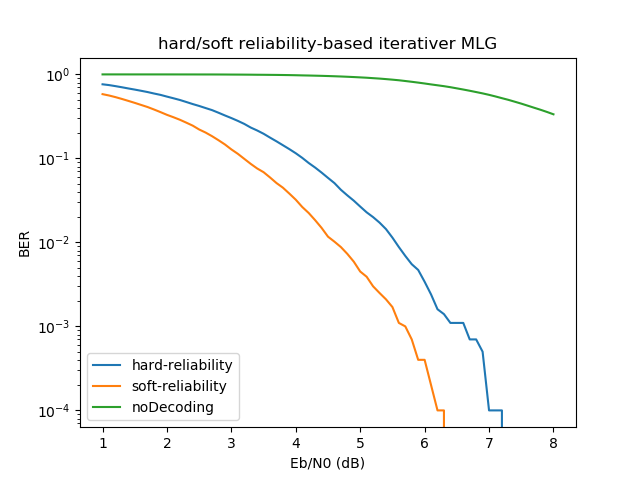
\includegraphics[width=\linewidth]{foo3.png}
	\caption{Revised - Vergleich soft- und hard-reliability-based iterativer MLG}
	\label{fig:plot2}
\end{figure}


\newpage

Die Leistungsfähigkeit des Kodes wurde für maximale Iterationen zwischen 2 und 10 Iterationsschritten getestet. Wie in Abbildung \ref{fig:iter} zu sehen, ist der Dekodierunsgewinn ab etwa 6 Iterationsschritten vernachlässigbar.\\

Die soft-reliability wurde mit einer angepassten 4-Bit-Quantisierung umgesetzt. Für diese ergibt sich $ 2^{x-1} - 1 = 2^{3} - 1 = 7 $.\\

\begin{figure}[ht]
	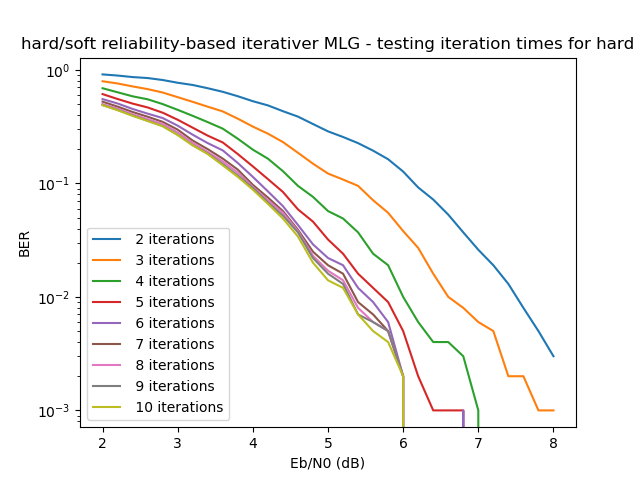
\includegraphics[width=\linewidth]{iter.png}
	\caption{Vergleich Dekodierverhalten hard-reliability-based iterativer MLG mit 2-10 Iterationsstufen}
	\label{fig:iter}
\end{figure} 

\paragraph{Auswertung}

Der soft-reliability iterative MLG bietet einen generellen Kodierungsgewinn von etwa 1 dB gegenüber dem hard-reliability iterative MLG.

\section{Umsetzung} Der Quellcode für die hier gezeigten Berechnungen ist auf github unter \url{https://github.com/Manonisch/Kanalkodierung} \href{https://github.com/Manonisch/Kanalkodierung}  abrufbar. Grundlage bildet Python mit den Bibliotheken Numpy und Matplotlib.


\section{Veraltet: Majority Logic-Decoder}

Anmerkung: dieser Abschnitt ist veraltet und dient lediglich als Refernen für den Abschnitt 'Korrektur Majority-Logic Decoder'.

Für die Untersuchung des hard/soft-reliability MLG Decoder wurde ein Kanal mit AWGN-Rauschen implementiert und eine Sample-Größe von jeweils 10000 übertragenen Wörtern getestet.
Die Rauschabstände wurden in 0,1 Schritten zwischen 1 und 8 dB gewählt. Abbildung \ref{fig:plot} zeigt die durchschnittliche Restfehlerwahrscheinlichkeit für den gegebenen Kode und maximal 12 Iterationen. Die soft-reliability wurde mit einer 9-Bit-Quantisierung umgesetzt. 

Der soft-reliability iterative MLG bietet vor allem für kleinere Rauschabstände zwischen 4 und 8 dB Vorteile gegenüber dem hard-reliability iterative MLG von 0,5 bis dB. 

\begin{figure}[hb]
	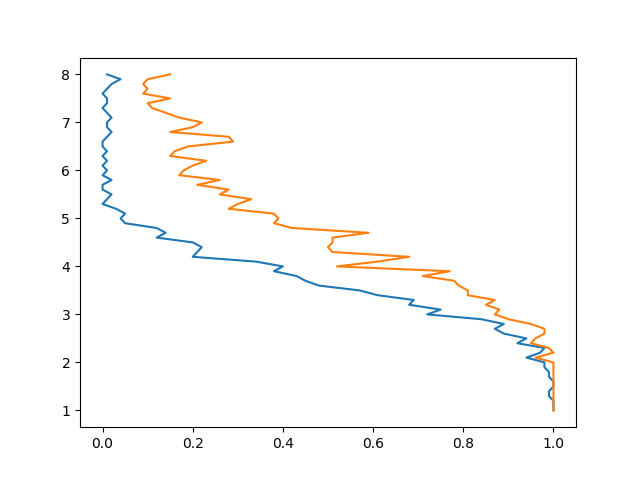
\includegraphics[width=\linewidth]{foo.png}
	\caption{veraltet: Vergleich soft- und hard-reliability-based iterativer MLG auf alter Programmbasis}
	\label{fig:plot}
\end{figure}


\paragraph{Anmerkungen} Während der Untersuchung fiel auf, dass die Anzahl der Quantisierungsstufen maßgeblich Einfluss auf die Korrektureigenschaft des soft-reliability iterative MLG hatte. Bei einer Menge an Quantisierungsstufen $x < \gamma $ mit $\gamma$ ist Spaltengewicht der Kontrollmatrix, war das Dekodierverhalten teils schlechter, als beim hard-reliability iterative MLG.

Wie im Graph zu sehen, liefert der Hard-reliability Algorithmus oberhalb eines Rauschabstandes von 6 DB konstante Werte an Restfehlerwahrscheinlichkeit ab, anstatt, wie erwartet gegen 0 zu gehen. Dieses Verhalten kann m.M.n. entweder auf einen bis dato unerkannten Fehler im Algorithmus oder aber auf das Auftreten eines ungünstigen Fehlermusters durch die Struktur der gegebenen Kontrollmatrix zurückgeführt werden. 


\end{document}